%!TEX root = <C++Report.tex>
\pgfdeclarelayer{edgelayer}
\pgfdeclarelayer{nodelayer}
\pgfsetlayers{edgelayer,nodelayer,main}

\tikzstyle{none}=[inner sep=0pt]

\tikzstyle{rn}=[circle,fill=Red,draw=Black,line width=0.8 pt]
\tikzstyle{gn}=[circle,fill=Lime,draw=Black,line width=0.8 pt]
\tikzstyle{yn}=[circle,fill=Yellow,draw=Black,line width=0.8 pt]
\tikzstyle{wn}=[rectangle,fill=White,draw=Black]
\tikzstyle{cxx}=[rectangle,fill=LightGreen,draw=Black]
\tikzstyle{hr}=[rectangle,fill=IndianRed,draw=Black]
\tikzstyle{newstyle}=[rectangle,fill=White,draw=White]

\tikzstyle{simple}=[-,draw=Black]
\tikzstyle{arrow}=[-latex,draw=Black]
\tikzstyle{tick}=[-,draw=Black,postaction={decorate},decoration={markings,mark=at position .5 with {\draw (0,-0.1) -- (0,0.1);}},line width=2.000]

\newlength{\imagewidth}
\newlength{\imagescale}

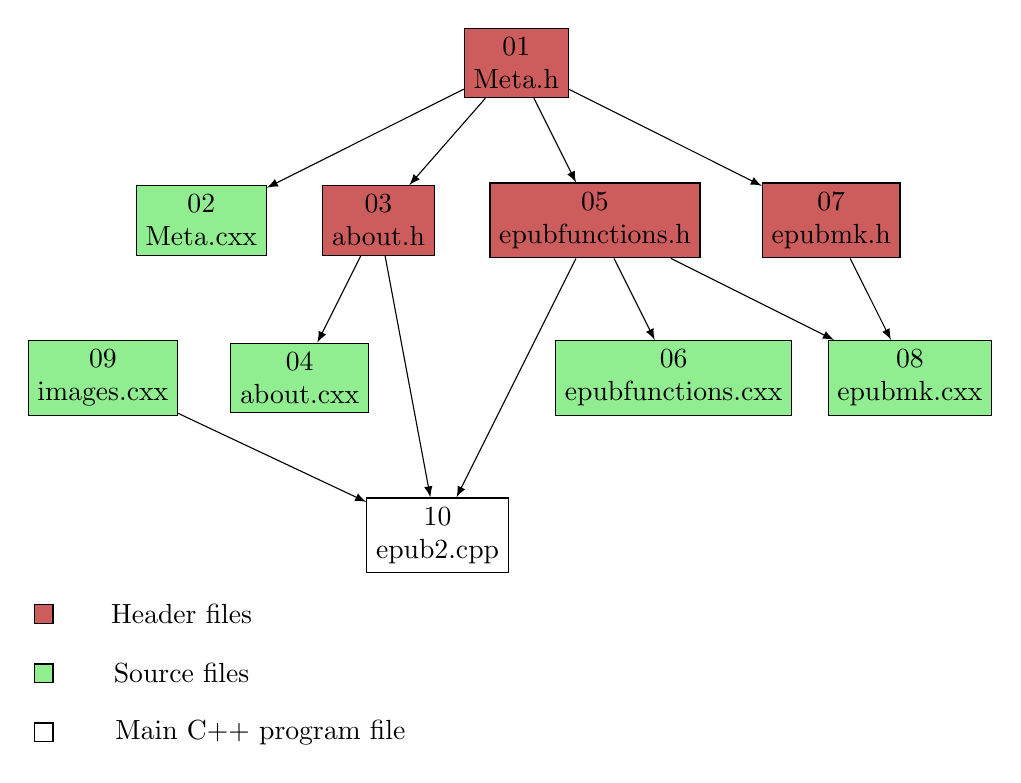
\begin{tikzpicture}
	\begin{pgfonlayer}{nodelayer}
		\node [style=hr] (0) at (0, -0) [align=center] {01\\Meta.h};
		\node [style=hr] (1) at (1, -2) [align=center] {05\\epubfunctions.h};
		\node [style=hr] (2) at (4, -2) [align=center] {07\\epubmk.h};
		\node [style=hr] (3) at (-1.75, -2) [align=center] {03\\about.h};
		\node [style=cxx] (4) at (2, -4) [align=center] {06\\epubfunctions.cxx};
		\node [style=cxx] (5) at (5, -4) [align=center] {08\\epubmk.cxx};
		\node [style=cxx] (6) at (-4, -2) [align=center] {02\\Meta.cxx};
		\node [style=cxx] (7) at (-2.75, -4) [align=center] {04\\about.cxx};
		\node [style=wn] (8) at (-1, -6) [align=center] {10\\epub2.cpp};
		\node [style=cxx] (9) at (-5.25, -4) [align=center] {09\\images.cxx};
		\node [style=hr] (10) at (-6, -7) {};
		\node [style=cxx] (11) at (-6, -7.75) {};
		\node [style=wn] (12) at (-6, -8.5) {};
		\node [style=newstyle] (13) at (-4.25, -7) {Header files};
		\node [style=newstyle] (14) at (-4.25, -7.75) {Source files};
		\node [style=newstyle] (15) at (-3.25, -8.5) {Main C++ program file};
	\end{pgfonlayer}
	\begin{pgfonlayer}{edgelayer}
		\draw [style=arrow] (0) to (2);
		\draw [style=arrow] (0) to (1);
		\draw [style=arrow] (0) to (3);
		\draw [style=arrow] (1) to (8);
		\draw [style=arrow] (1) to (4);
		\draw [style=arrow] (1) to (5);
		\draw [style=arrow] (0) to (6);
		\draw [style=arrow] (3) to (7);
		\draw [style=arrow] (3) to (8);
		\draw [style=arrow] (9) to (8);
		\draw [style=arrow] (2) to (5);
	\end{pgfonlayer}
\end{tikzpicture}
